\chapter{Zbieranie i przetwarzanie danych z czujników}

\section*{Raspberry Pi}

Wszystkie zestawy zbudowaliśmy w oparciu o Raspberry Pi 3 v1.2. Zdecydowaliśmy się na to rozwiązanie, ponieważ bazuje on na dystrybucji Linuxa, posiada opowiednie interfejsy i złącza a także zintegrowany moduł WiFi. Minusem w stosunku do konkurencyjnego Arduino jest brak wejść analogowych. Problem rozwiązano dodając zewnętrzny przetwornik A/C.
\paragraph{Specyfikacja Raspberry Pi 3:}
\begin{itemize} 
\item Procesor 1.2 GHz
\item Liczba rdzeni 4. Quad Core
\item Pamięć RAM 1 GB
\item Pamięć Karta microSD
\item 40 GPIO
\end{itemize}
\begin{figure}[h]
	\centering
	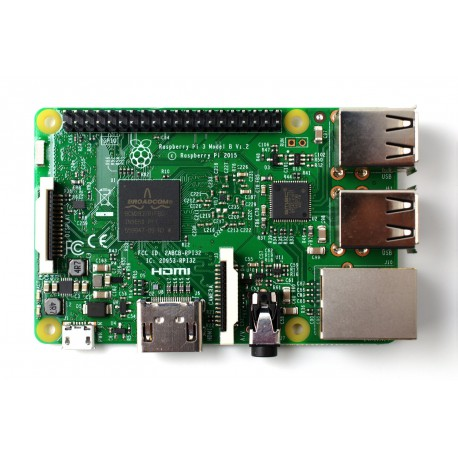
\includegraphics[width=6cm]{raspberry.jpg}
	\caption{Raspberry Pi 3}
\end{figure}
Aby prawidłowo zainstalować oprogramowanie The Guard na dowolnym urządzeniu Raspberry Pi 3 należy wykonać poniższe czynności w terminalu:
\begin{enumerate} 
\item sudo apt-get install libx264-dev
\item cd /usr/src
\item git clone git://source.ffmpeg.org/ffmpeg.git
\item sudo ./configure --arch=armel --target-os=linux --enable-gpl --enable-libx264 --enable-nonfree
\item sudo make
\item sudo install
\item sudo nano /boot/config.txt
\item dopisać w pliku Dtoverlay=w1-gpio i Gpiopin=4
\item pip intall wiringpi
\item sudo pip install spidev
\item pip install pyrebase
\end{enumerate}
Następnym krokiem jest włączenie odpowiednich interfejsów w panelu konfiguracyjnym. Należy zmienić ustawienia zgodnie z poniższym schematem:

\begin{figure}[h]
	\centering
	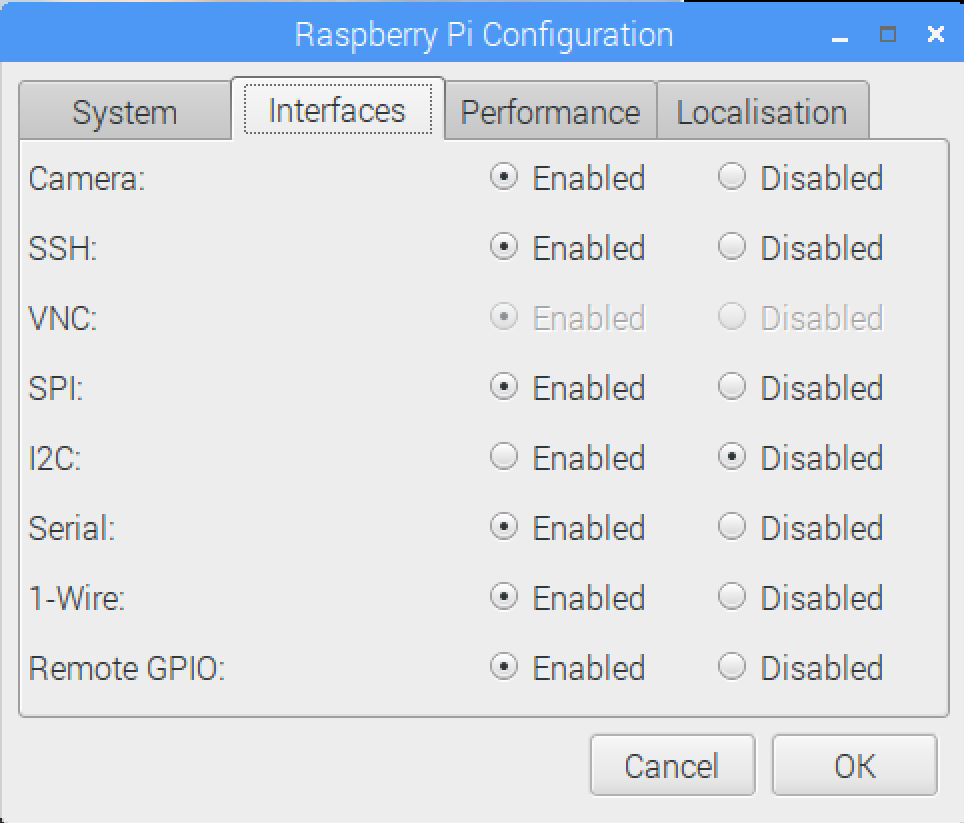
\includegraphics[width=6cm]{RSettings}
	\caption{Ustawienia}
\end{figure}

W kodzie używamy biblioteki wiringpi do odczytu danych z układów cyfrowych. Należy zaznaczyć, że numeracja fizycznych pinów i numeracja pinów w bibliotece wiringPi jest różna i nie zawiera wszystkich dostępnych pinów na urządzeniu. 

\begin{figure}[h]
  \centering
  \begin{minipage}[b]{0.4\textwidth}
    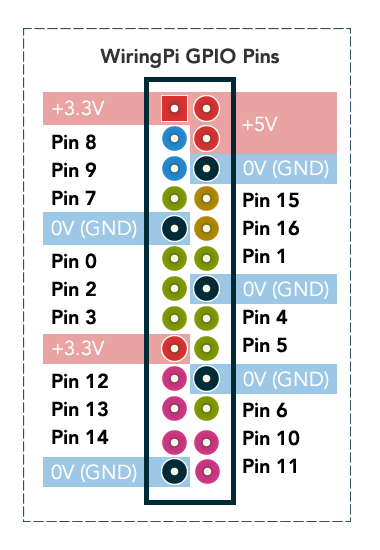
\includegraphics[width=\textwidth]{wiringpi.png}
    \caption{WiringPi}
  \end{minipage}
  \hfill
  \begin{minipage}[b]{0.4\textwidth}
    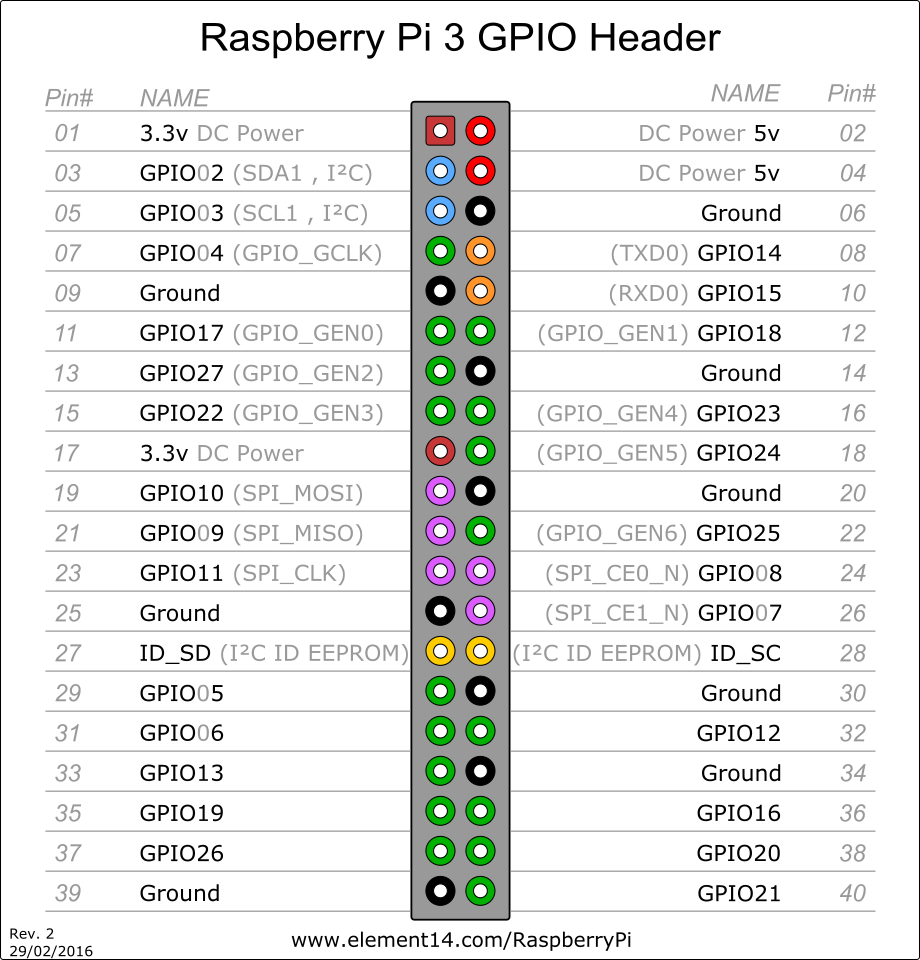
\includegraphics[width=\textwidth]{gpio.png}
    \caption{GPIO}
  \end{minipage}
\end{figure}

\section*{Czujniki}

Lista i opis, schematy, kod

\section*{Obsługa wideo}

Opis procesu, opis Nginxa, opis RTMP i HLS